\documentclass[tikz,border=2pt]{standalone}
\usepackage{amsmath,amssymb}
\usepackage{pgfplots}
\pgfplotsset{compat=1.18}

\begin{document}
% ||x||_∞ = max(|x1|,|x2|): the "unit circle" is the square with corners (±1,±1); the point
% (0.6, -1) has maximum norm 1, decided by its larger coordinate.
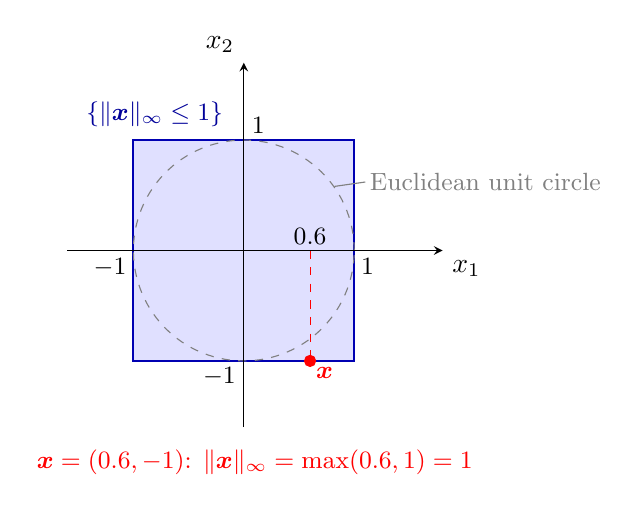
\begin{tikzpicture}
	\begin{axis}[
		axis lines=middle, axis equal image, axis on top,
		xmin=-1.6, xmax=1.8, ymin=-1.6, ymax=1.7,
		xtick=\empty, ytick=\empty,
		xlabel={$x_1$}, ylabel={$x_2$},
		xlabel style={below right}, ylabel style={above left},
		clip=false, width=7.2cm
		]
		\fill[blue!12] (axis cs:-1,-1) rectangle (axis cs:1,1);
		\draw[thick, blue!70!black] (axis cs:-1,-1) rectangle (axis cs:1,1);
		\addplot[gray, dashed, domain=0:360, samples=120] ({cos(x)}, {sin(x)});
		\addplot[only marks, mark=*, red] coordinates {(0.6,-1)};
		\draw[dashed, red] (axis cs:0.6,0) -- (axis cs:0.6,-1);
		\node[anchor=north west, font=\small, inner sep=1.5pt] at (axis cs:1.02,-0.03) {$1$};
		\node[anchor=north east, font=\small, inner sep=1.5pt] at (axis cs:-1.02,-0.03) {$-1$};
		\node[anchor=south west, font=\small, inner sep=1.5pt] at (axis cs:0.03,1.02) {$1$};
		\node[anchor=north east, font=\small, inner sep=1.5pt] at (axis cs:-0.03,-1.02) {$-1$};
		\node[anchor=south, font=\small, inner sep=2pt] at (axis cs:0.6,0) {$0.6$};
		\node[red, anchor=north west, font=\small, inner sep=2pt] at (axis cs:0.6,-1) {$\boldsymbol{x}$};
		\node[blue!60!black, anchor=south east, font=\small] at (axis cs:-0.1,1.03) {$\{\|\boldsymbol{x}\|_\infty\le 1\}$};
		\draw[gray, thin] (axis cs:0.82,0.58) -- (axis cs:1.1,0.62);
		\node[gray, anchor=west, font=\small, inner sep=1.5pt] at (axis cs:1.1,0.62) {Euclidean unit circle};
		\node[red, anchor=north, font=\small] at (axis cs:0.1,-1.72) {$\boldsymbol{x}=(0.6,-1)$: $\|\boldsymbol{x}\|_\infty=\max(0.6,1)=1$};
	\end{axis}
\end{tikzpicture}
\end{document}
